\begin{figure*}[t]                 
	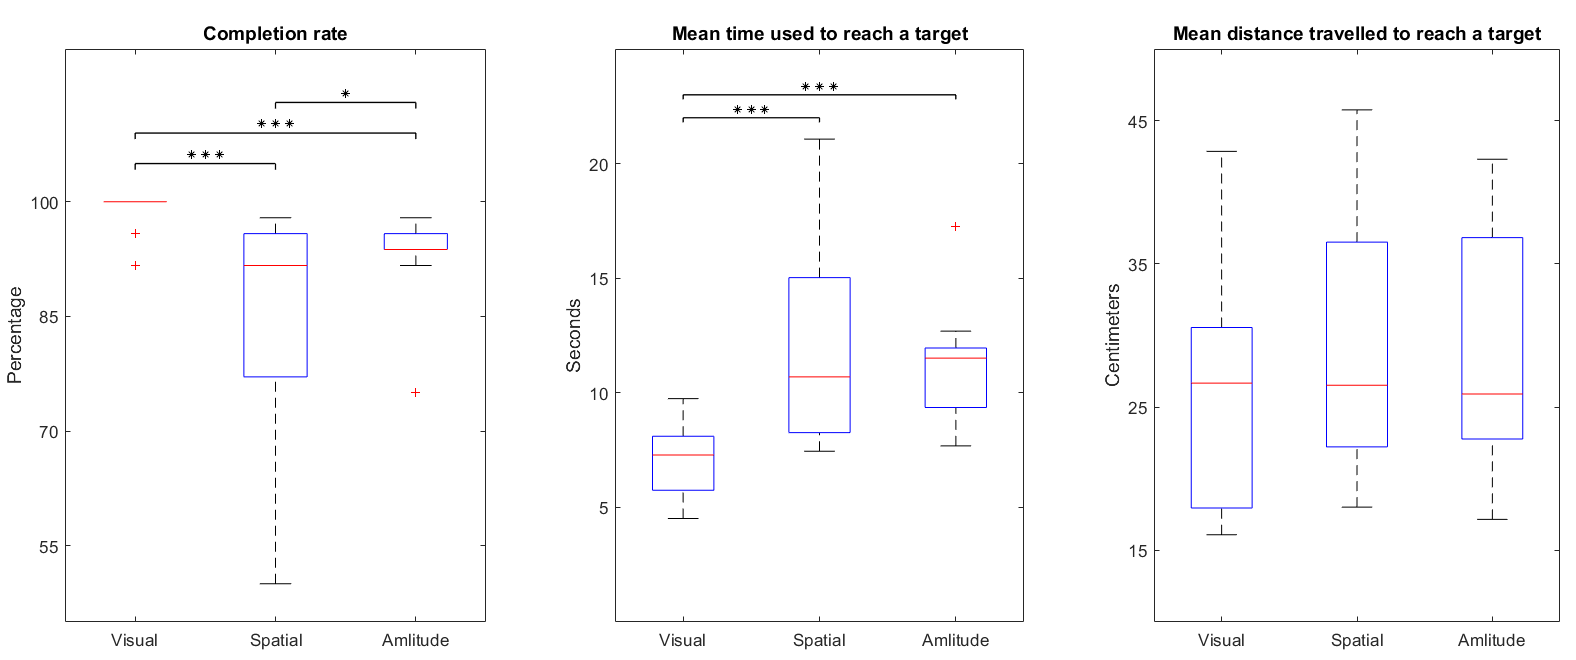
\includegraphics[width=.8\textwidth]{figures/boxplot_results}
	\caption{Box plots of the metrics extracted from the visual, spatial and amplitude feedback evaluation tests. The two evaluation tests in the spatial and amplitude feedback block, respectively, were combined by calculating the mean between the two tests.}
	\label{fig:pa:boxplot_results} 
\end{figure*}

\begin{figure*}[t]                 
	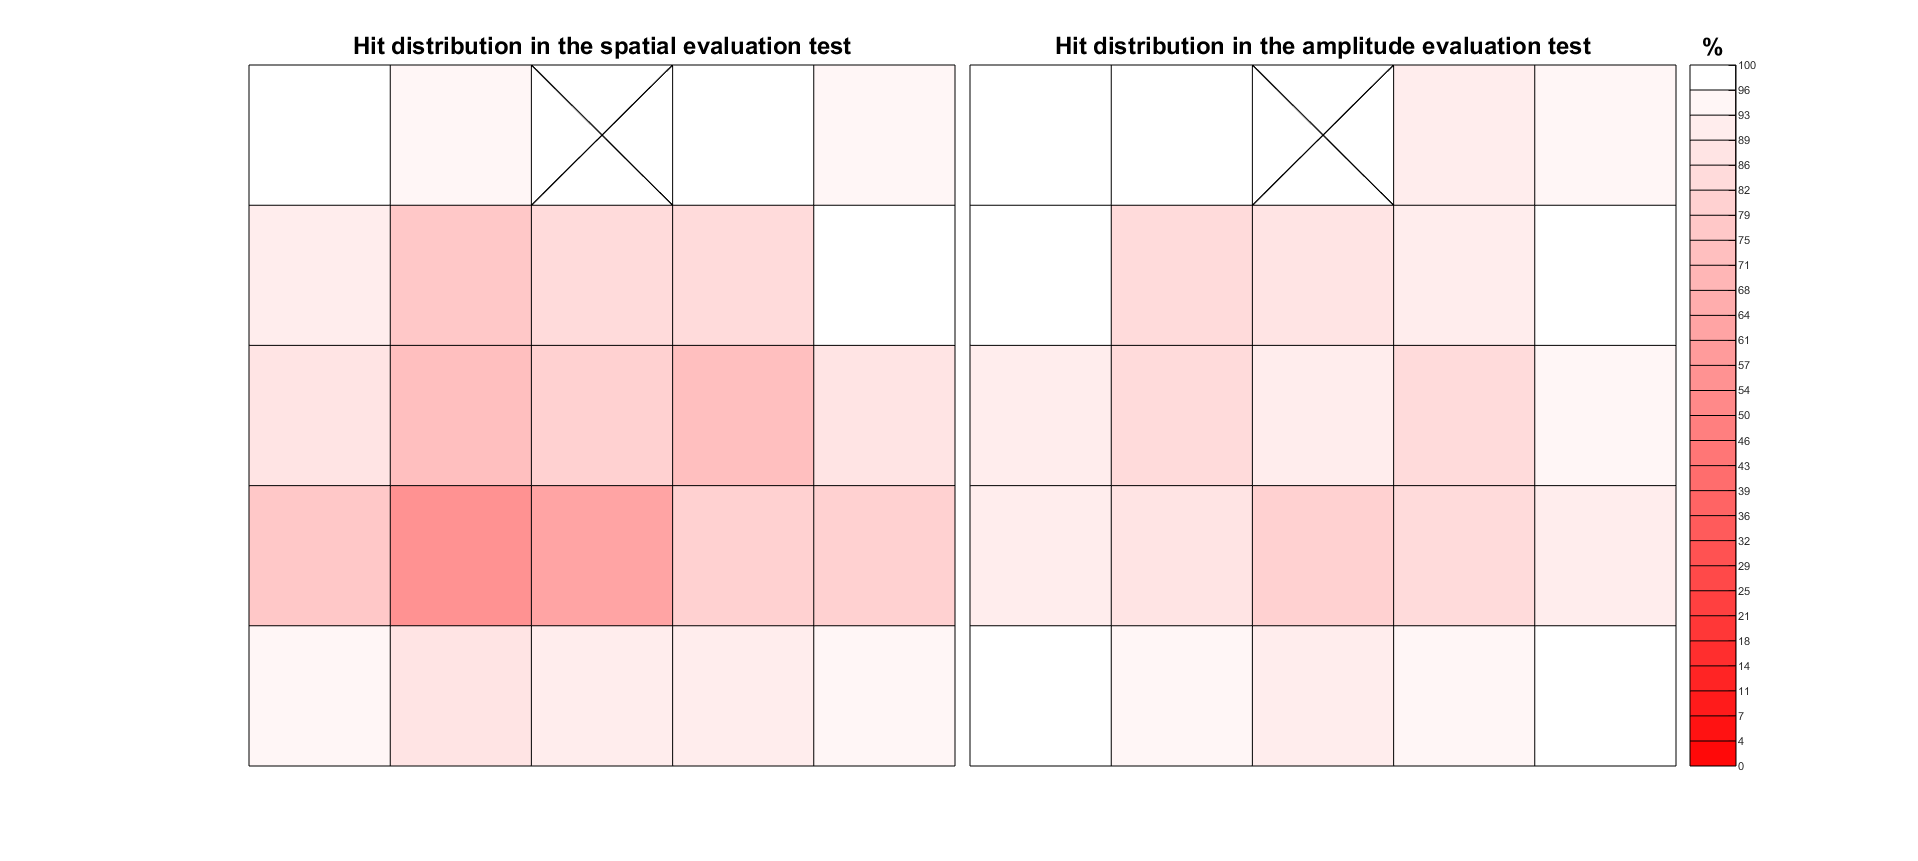
\includegraphics[width=.8\textwidth]{figures/hit_dist}
	\caption{Hit rate for each target in the spatial and amplitude evaluation test, respectively. The more transparent a target is, the higher the hit rate was.}
	\label{fig:pa:hit_dist} 
\end{figure*}
Due to yielding no significant difference (p > 0.05) between the two evaluation tests for both the spatial and amplitude feedback block, it was chosen to view these evaluation tests as one, by calculating the mean between the two tests in both blocks. Figure \ref{fig:pa:boxplot_results} shows box plots of the extracted metrics for the visual, spatial and amplitude feedback evaluation tests. Worth noting was that visual feedback still outperformed solely relying on electrotactile feedback both when spatially or amplitude modulated for the completion rate and time to reach a target metrics. When comparing the spatial and amplitude feedback tests, using amplitude feedback yielded a slightly higher completion rate (p = 0.044). This quantitative result was also supported by the subjective opinion of the subjects as 64 \% of the subjects favoured the amplitude feedback. However, all subjects struggled in choosing a favoured feedback scheme as they found both intuitive to understand. 

When observing the completion rate of the specific targets in figure \ref{fig:pa:hit_dist}, it can be derived that targets generally had a higher hit rate when using amplitude feedback compared to spatial. However, common for both feedback scheme was that the centred targets were more troublesome to reach (maybe note completion rate for centred vs outer targets). A possible reason for this finding is that the subjects had to achieve complete rest to dwell inside these targets. In the outer targets, the subjects did not necessarily need to achieve complete rest, as they could continue performing a movement and still be on the boundary of the target. Furthermore, combined DoF targets generally had a lower completion rate for both feedback schemes (maybe note the completion rate of single DoF targets vs combined). This could indicate that the sensory feedback regarding combined prosthetic states were harder to interpret. (Mean completion rate in spatial = 87 \% and amplitude = 93 \%)


